\chapter{TDD}

\section{Tensor Decision Diagrams(TDD)介绍}
\begin{itemize}
  \item 张量网络表示量子线路
  \item 张量决策图
  \item TDD的规范与化简
\end{itemize}
% //TODO: add some
\subsubsection{张量网络表示量子线路}
张量是与一组与索引\(I=\{x_1,\ldots,x_n\}\)相关联的多维线性映射。在量子计算中,可以假设只从\(\{0,1\}\)中取值。因此,张量定义为:
\begin{align}
    \phi :{\{0,1\}}^I\rightarrow\mathbb{C}
\end{align}
其中\(\mathbb{C}\)为实数。张量网络是一个无向图\(G=\left(V,E\right)\)。其中顶点集V中的每个顶点v表示一个张量。边集\(E\)中每条边\(e\)代表与相邻两个张量相关联的公共索引。通过以任意顺序收缩连接的张量,可以得到一个秩为\(m\)的张量,其中\(m\)是$G$中开放边数。这个独立于收缩顺序的张量也称为该张量网络的张量表示\citep{biamonte2019lectures}。
张量网络提供了一种新的量子线路表示方法\citep{pednault2017breaking}。一个向量表示为$[\alpha_0,\alpha_1]$的量子比特x可以描述为秩为1的张量$\phi_x$,其中$\phi_x\left(0\right)=\alpha_0, \phi_x\left(1\right)=\alpha_1$。具有输入比特x和输出比特y的单比特门可以表示为秩2张量$\phi_{xy}$。例如,以x作为输入比特和y作为输出比特的单比特门Z-gate的张量表示:$\phi_{xy}\left(00\right)=1,\phi_{xy}\left(01\right)=\phi_{xy}\left(10\right)=0,\phi_{xy}\left(11\right)=-1$。类似的$n$比特量子门可以表示成一个秩为$2n$的张量。在张量表示中,一般不区分输入和输出索引。只有当将张量解释为门或电路时会规定关于其信息。

给定量子线路中所有量子门的输入和输出状态的索引值,就可以得到量子电路的张量表示。图\ref{fig:example_cir_map}给定了图\ref{fig:example_cir}中量子线路中各个状态的索引值,从而可得的张量表示:
\begin{align}
\phi_{x_0x_3y_0y_3}\left(a_0a_3b_0b_3\right)=\sum_{a_1,a_2,b_1,b_2=0}^{1}T\left(a_0a_1\right)H\left(b_0b_1\right)CX\left(a_1b_1a_2b_2\right)T\left(a_2a_3\right)H\left(b_2b_3\right)
\end{align}

\begin{figure}[!htbp]
    \centering
    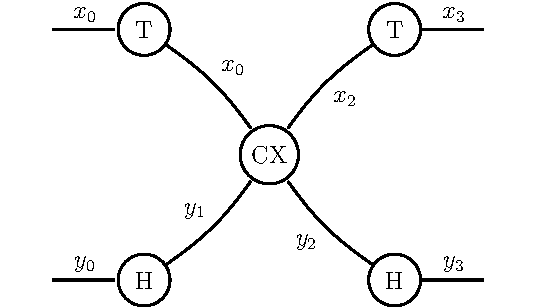
\includegraphics[width=.6\textwidth]{Img/tensor_example.pdf}
    \caption{用张量表示图\ref{fig:example_cir}中量子线路}   
    \label{fig:example_cir_map}
\end{figure}

\subsubsection{张量决策图}
张量决策图(Tensor Decision Diagrams,或TDD)是一种具有决策图和张量网络特征的数据结构\citep{Hong_2022}。它可用于表示张量和量子电路。与BDD(Boolean Decision Diagrams)类似,TDD是一种建立在索引顺序$I=\{x_1,\ldots,x_n\}$上的决策树模型。具体定义如下:
\begin{align}
    \mathcal{F}=\left(V,E,index,value,low,high,w\right)
\end{align}
其中$V$是一个有限节点集,被划分为非终端节点$V_n$和终端节点$V_T$。用$r_{\mathcal{F}}$表示$\mathcal{F}$的唯一根节点。$E=\left\{\left(v,low\left(v\right)\right),\left(v,high\left(v\right)\right):v\in V_N\right\}$是树中所有边集合,其中$\left(v,low\left(v\right)\right)$和$\left(v,high\left(v\right)\right)$分别称为v的低边和高边。根结点$r_{\mathcal{F}}$具有唯一的入射边$e_{\mathcal{F}}$,该入射边没有源结点。$index:V_r\rightarrow I$将每个非终端节点分配给I中的索引。$value:V_T\rightarrow\mathbb{C}$将每个终端节点赋予一个复数值。$low$和$high$都是$V_N\rightarrow V$中的映射,它们分别为每个非终端节点指定其低边和高边后继。$w:E\rightarrow\mathbb{C}$将每条边赋予一个复数权重。特别地,$w\left(e_r\right)$称为$\mathcal{F}$的权重,并记作$w_{\mathcal{F}}$。 



图\ref{fig:tdd_ex} 展示了一个TDD的例子。其中索引顺序$I=\{x_0,y_0,y_3\}$。非终端节点$V_n$用圆表示,终端节点$V_T$用方形表示。每个节点的低边用虚线表示,高边用实线表示。该示例中各边的权重均为1,即$w:E\rightarrow 1$。根节点$r_{\mathcal{F}}=x_0$。决策树的权重$w_{\mathcal{F}}=1$。
\begin{figure}[!htbp]
    \centering
    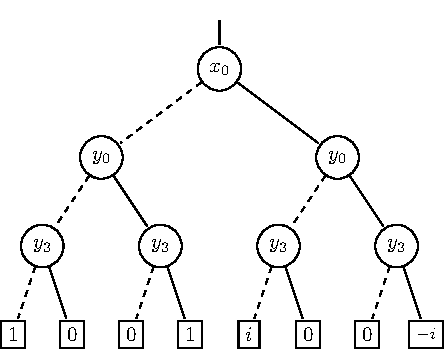
\includegraphics[width=.6\textwidth]{Img/tree_tdd.pdf}
    \caption{一个TDD示例}   
    \label{fig:tdd_ex}
\end{figure}

对于TDD中的一个节点$v$,如果$v$是终端节点,则$\phi\left(v\right):= valuev$是一个秩为$0$的张量,即常数。如果$v$是非终端节点,则:
\begin{align}
    \phi(v):=w_{0} \cdot \overline{x_{v}} \cdot \phi(\operatorname{low}(v))+w_{1} \cdot x_{v} \cdot \phi(h i g h(v))
\end{align}
其中$x_v=index\left(v\right),\bar{x_v}=1-index\left(v\right)$。如果$v$是非终端节点,也可以表示为:
\begin{align}
    \left.\phi\left(v\right)\right|_{x_v=c}≔w_c \phi (v_c)
\end{align}
其中$c\in\{0,1\}$。因此整个TDD也可以表示为:
\begin{align}
    \phi\left(\mathcal{F}\right)=w_{\mathcal{F}}\cdot\phi\left(r_{\mathcal{F}}\right)
\end{align}
\subsubsection{TDD的规范与化简}
对于图表 6中的TDD,在结构上显然比较冗余。因此可以先进行规范化(normalized),让后进行化简(reduced)\citep{Hong_2022}。
规范化的目的是使得TDD的终端节点只包含0和1,同时将终端节点的张量值沿路径逐步上移。具体规范步骤如下:
\begin{myen}
    \item 如果$v$是一个非零值$value\left(v\right)\neq 1$的终端节点,则将其值设置为1,并将每个入边的权重w更改为$value\left(v\right)\cdot w$。\label{norm1}
    \item 假设v是一个非终端节点,且$\phi\left(v\right)\neq 0$。首先规范化$\phi\left.\left(low(v\right)\right)$和$\phi\left.\left(high(v\right)\right)$。完成$\phi\left.\left(low(v\right)\right)$和$\phi\left.\left(high(v\right)\right)$的规范化后。如果$\phi\left.\left(low(v\right)\right)\neq 0$,并且此时$\phi\left.\left(high(v\right)\right)=0$或$\left|w_0\right|\geq\left|w_1\right|$,则将$w$设置为$w_0$。否则,将$w$设置为$w_1$。然后更新$w_0≔w_0/w,w_1≔w_1/w$。此时完成$v$的规范化。\label{norm2}
\end{myen}

\begin{figure}[!htbp]
    \centering
    \begin{subfigure}[b]{0.4\textwidth}
        \centering
        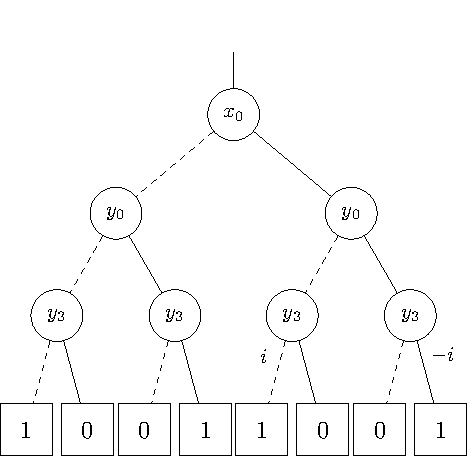
\includegraphics[height=5cm]{Img/tree_norm1.pdf}
        \caption{对图\ref{fig:tdd_ex}的终端节点规范化}
        \label{fig:tdd-norma}
    \end{subfigure}
    \begin{subfigure}[b]{0.4\textwidth}
        \centering
        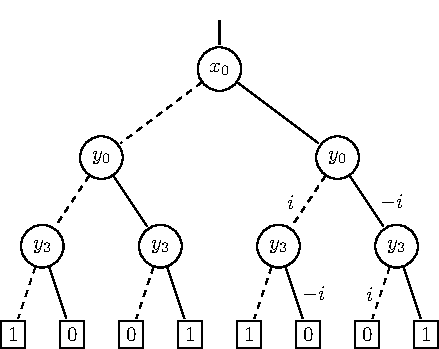
\includegraphics[height=5cm]{Img/tree_norm2.pdf}
        \caption{对图\ref{fig:tdd-norma}的$y_3$节点规范化}
        \label{fig:tdd-normb}
    \end{subfigure}
    \\
    \begin{subfigure}[b]{0.8\textwidth}
        \centering
        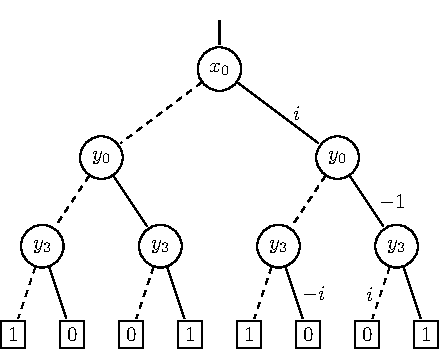
\includegraphics[width=.8\textwidth]{Img/tree_norm3.pdf}
        \caption{对图\ref{fig:tdd_ex}的规范化结果}
        \label{fig:tdd-normc}
    \end{subfigure}
    % \caption{对图\ref{fig:tdd_ex}的规范化过程}
    \label{fig:tdd-norm}
\end{figure}
对于图\ref{fig:tdd_ex}中的TDD。具体规范化过程为:应用第\ref{norm1}步于$i$和$-i$两个终端节点得到图表 \ref{fig:tdd-norma};然后,应用第\ref{norm2}步于右侧两个$y_3$节点,得到图表 \ref{fig:tdd-normb};最后,应用第二条规则于于右侧$y_0$节点。最后可以获得图表 \ref{fig:tdd-normc}。

在完成规范化后,可以进一步简化TDD,使得TDD只包含一个终端节点,同时尽量使用重复出现的张量。具体简化步骤如下:
\begin{myen}
    \item 	合并所有值为1的终端节点。删除所有终端$0$节点,并将它们的入边重定向到唯一的终端节点,并将它们的权重重置为$0$。\label{sympl1}
	\item 将所有权重为$0$的边重定向到终端节点。如果根节点的入边权重为$0$,则终端节点成为新的根,该TDD为空。删除所有从根节点不可达的节点,以及涉及它们的所有边。\label{sympl2}
	\item 如果一个节点v的低边和高边后继相同,并且其低边和高边具有相同的权重w,则删除该节点。如果入边权重$w=0$,则将其传入边重定向到终端节点。否则,将其传入边重定向到其后继节点。\label{sympl3}
	\item 合并两个具有相同索引、相同$0$和$1$后继以及对应边上相同权重的节点。\label{sympl4}
\end{myen}

\begin{figure}[!htbp]
    \centering
    \begin{subfigure}[b]{0.4\textwidth}
        \centering
        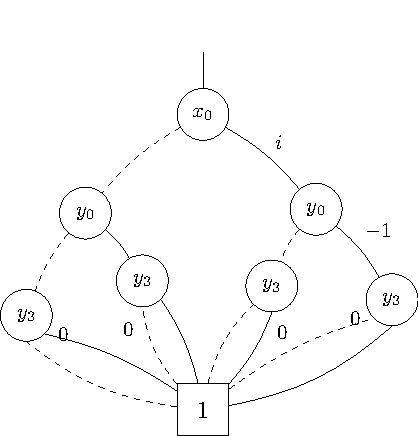
\includegraphics[height = 6cm]{Img/tree_redu1.pdf}
        \caption{对\ref{fig:tdd-normc}中规范TDD的终端节点化简}
        \label{fig:tdd-redu1}
    \end{subfigure}
    \begin{subfigure}[b]{0.4\textwidth}
        \centering
        \includegraphics[height = 6cm]{Img/tree_redu2.pdf}
        \caption{对图\ref{fig:tdd-normc}中规范TDD的简化结果}
        \label{fig:tdd-redu2}
    \end{subfigure}
    \label{fig:tdd-redu}
\end{figure}

对于图\ref{fig:tdd-normc}中规范TDD。具体化简过程为:首先重复第\ref{sympl1} 步,合并所有终端节点,得到图\ref{fig:tdd-redu1};由于没有符合第\ref{sympl2}和第\ref{sympl3}步的节点,因此直接进行第\ref{sympl4}步应用重复第四条规则合并第一个和第三个$y_3$节点,以及第二个和第四个$y_3$节点。最终可以得到\ref{fig:tdd-redu2}所示的简化TDD。

下文中所有的TDD均指化简后的TDD,即reduced tensor decision diagrams。

\subsection{在模型检验中应用TDD}
借助新的数据结构TDD,我们可以更方便的表示量子状态以及量子线路,并计算最终的结果。TDD给出了量子电路的紧凑表示,提供了一种方便的实现张量网络各种操作的方式,这些操作对于模拟量子物理系统非常重要。图表 12展示了一个矩阵和TDD形式,其中TDD中的蓝边表示高边,红边表示低边。可以明显看到TDD的结构更紧凑。
 	 
\begin{figure}[!htbp]
    \begin{subfigure}[c]{0.4\textwidth}
        \centering
        \includegraphics[width=\textwidth]{Img/matrix_of_tdd.pdf}
        \caption{矩阵$P$的矩阵形式}
        \label{fig:mat_P}
    \end{subfigure}
    \begin{subfigure}[c]{0.4\textwidth}
        \centering
        \includegraphics[height=6cm]{Img/tdd_ex.pdf}
        \caption{矩阵$P$的TDD形式}
        \label{fig:tdd_P}
    \end{subfigure}
\end{figure}

TDD特别适用于实现可达性分析和模型检查算法。这是因为基于BDD的模型检查算法中使用的许多优化技术可以推广到收缩量子电路张量网络上\citep{Chaki_2018}。这些为应用TDD解决量子模型检测问题提供了可能的方案。

\section{技术实施方案}
\begin{itemize}
  \item 索引顺序
  \item limdd
  \item addition的拆分方案
  \item contraction的拆分方案
\end{itemize}
% //TODO:modify here
% //TODO: add new paper
本次研究的主要目的是借助TDD数据结构,构建能快速计算量子模型检测中可达问题的方案。本次研究的主要挑战在于尽可能减少程序的运行时间以及空间资源。为此,需要采用一系列方法来开发更有效的算法,以优化TDD操作和收缩张量网络。其中包括开发新技术来分割张量网络和优化TDD结构。
下面简单介绍以下具体研究方法。

\begin{myen}

\item \label{addition}关于常用的量子线路划分方法,
第一种被称为addition\citep{chen2018classical}。将量子电路视为张量网络,首先将一个量子电路C转换成无向图G。G中的每个节点表示量子电路的一个索引,并且如果它们是相同门的输入或输出索引,则在G中连接两个节点。并且当满足以下两个条件之一时输入和输出索引不变:
\begin{itemize}
	\item 是对角线量子门的输入和输出索引;
	\item 是受控门的控制比特位的输入和输出索引。
\end{itemize}
	
图\ref{fig:addition}展示了Grover\_3电路图的索引链接图。该图描述了量子电路的连通性,通过选择图中连通度最大的索引可以对电路进行分割。因此选择图中连通度较大的$x_1^1,x_1^3x_2^1$可以对电路进行较好的划分。
 
\begin{figure}[!htbp]
	\centering
	\includegraphics[height=6cm]{Img/cir_index_graph.pdf}
	\caption{Grover\_3的索引连接图}
	\label{fig:addition}
\end{figure} 

\item 另一种常用的电路划分方法成为contraction。在这一方法中,将量子电路划分为若干个较小的部分,其收缩等于原始电路。对于两个预设整数参数k1和k2,将电路划分为若干小电路。其中每个小电路涉及最多k1个量子比特,并且与至多跨越不同部件的k2个多比特门相连。图\ref{fig:contraction}展示了对Bit flip电路进行k1=3,k2=2的拆分结果。
\begin{figure}[!htbp]
	\centering
	\includegraphics[height=7cm]{Img/cir_contraction.pdf}
	\caption{对Bit flip电路进行contraction的拆分}
	\label{fig:contraction}
\end{figure} 


\item \label{contraction}在BDD中,索引的顺序很重要。因为索引顺序会直接影响BDD的大小。一个良好的变量顺序可以使得BDD比一个糟糕的变量顺序小得多。图\ref{fig:bdd-compare}的了两张图都表示了布尔函数ƒ(x1,...,x8)=x1x2+x3x4+x5x6+x7x8,但图\ref{fig:bdd-good}的结构更简单。其中图\ref{fig:bdd-bad}的索引顺序为\{x1,x3,x5,x7,x2,x4,x6,x8\},图\ref{fig:bdd-good}的索引顺序为\{x1,x2,x3,x4,x5,x6,x7,x8\}。找到一个好的索引顺序是一个NP问题。在工程实现中,目前只能通过小规模电路上寻求规律,然后在更大规模电路中应用较优顺序。

\begin{figure}[!htbp]
	\centering
	\begin{subfigure}[b]{.4\textwidth}
        \centering
        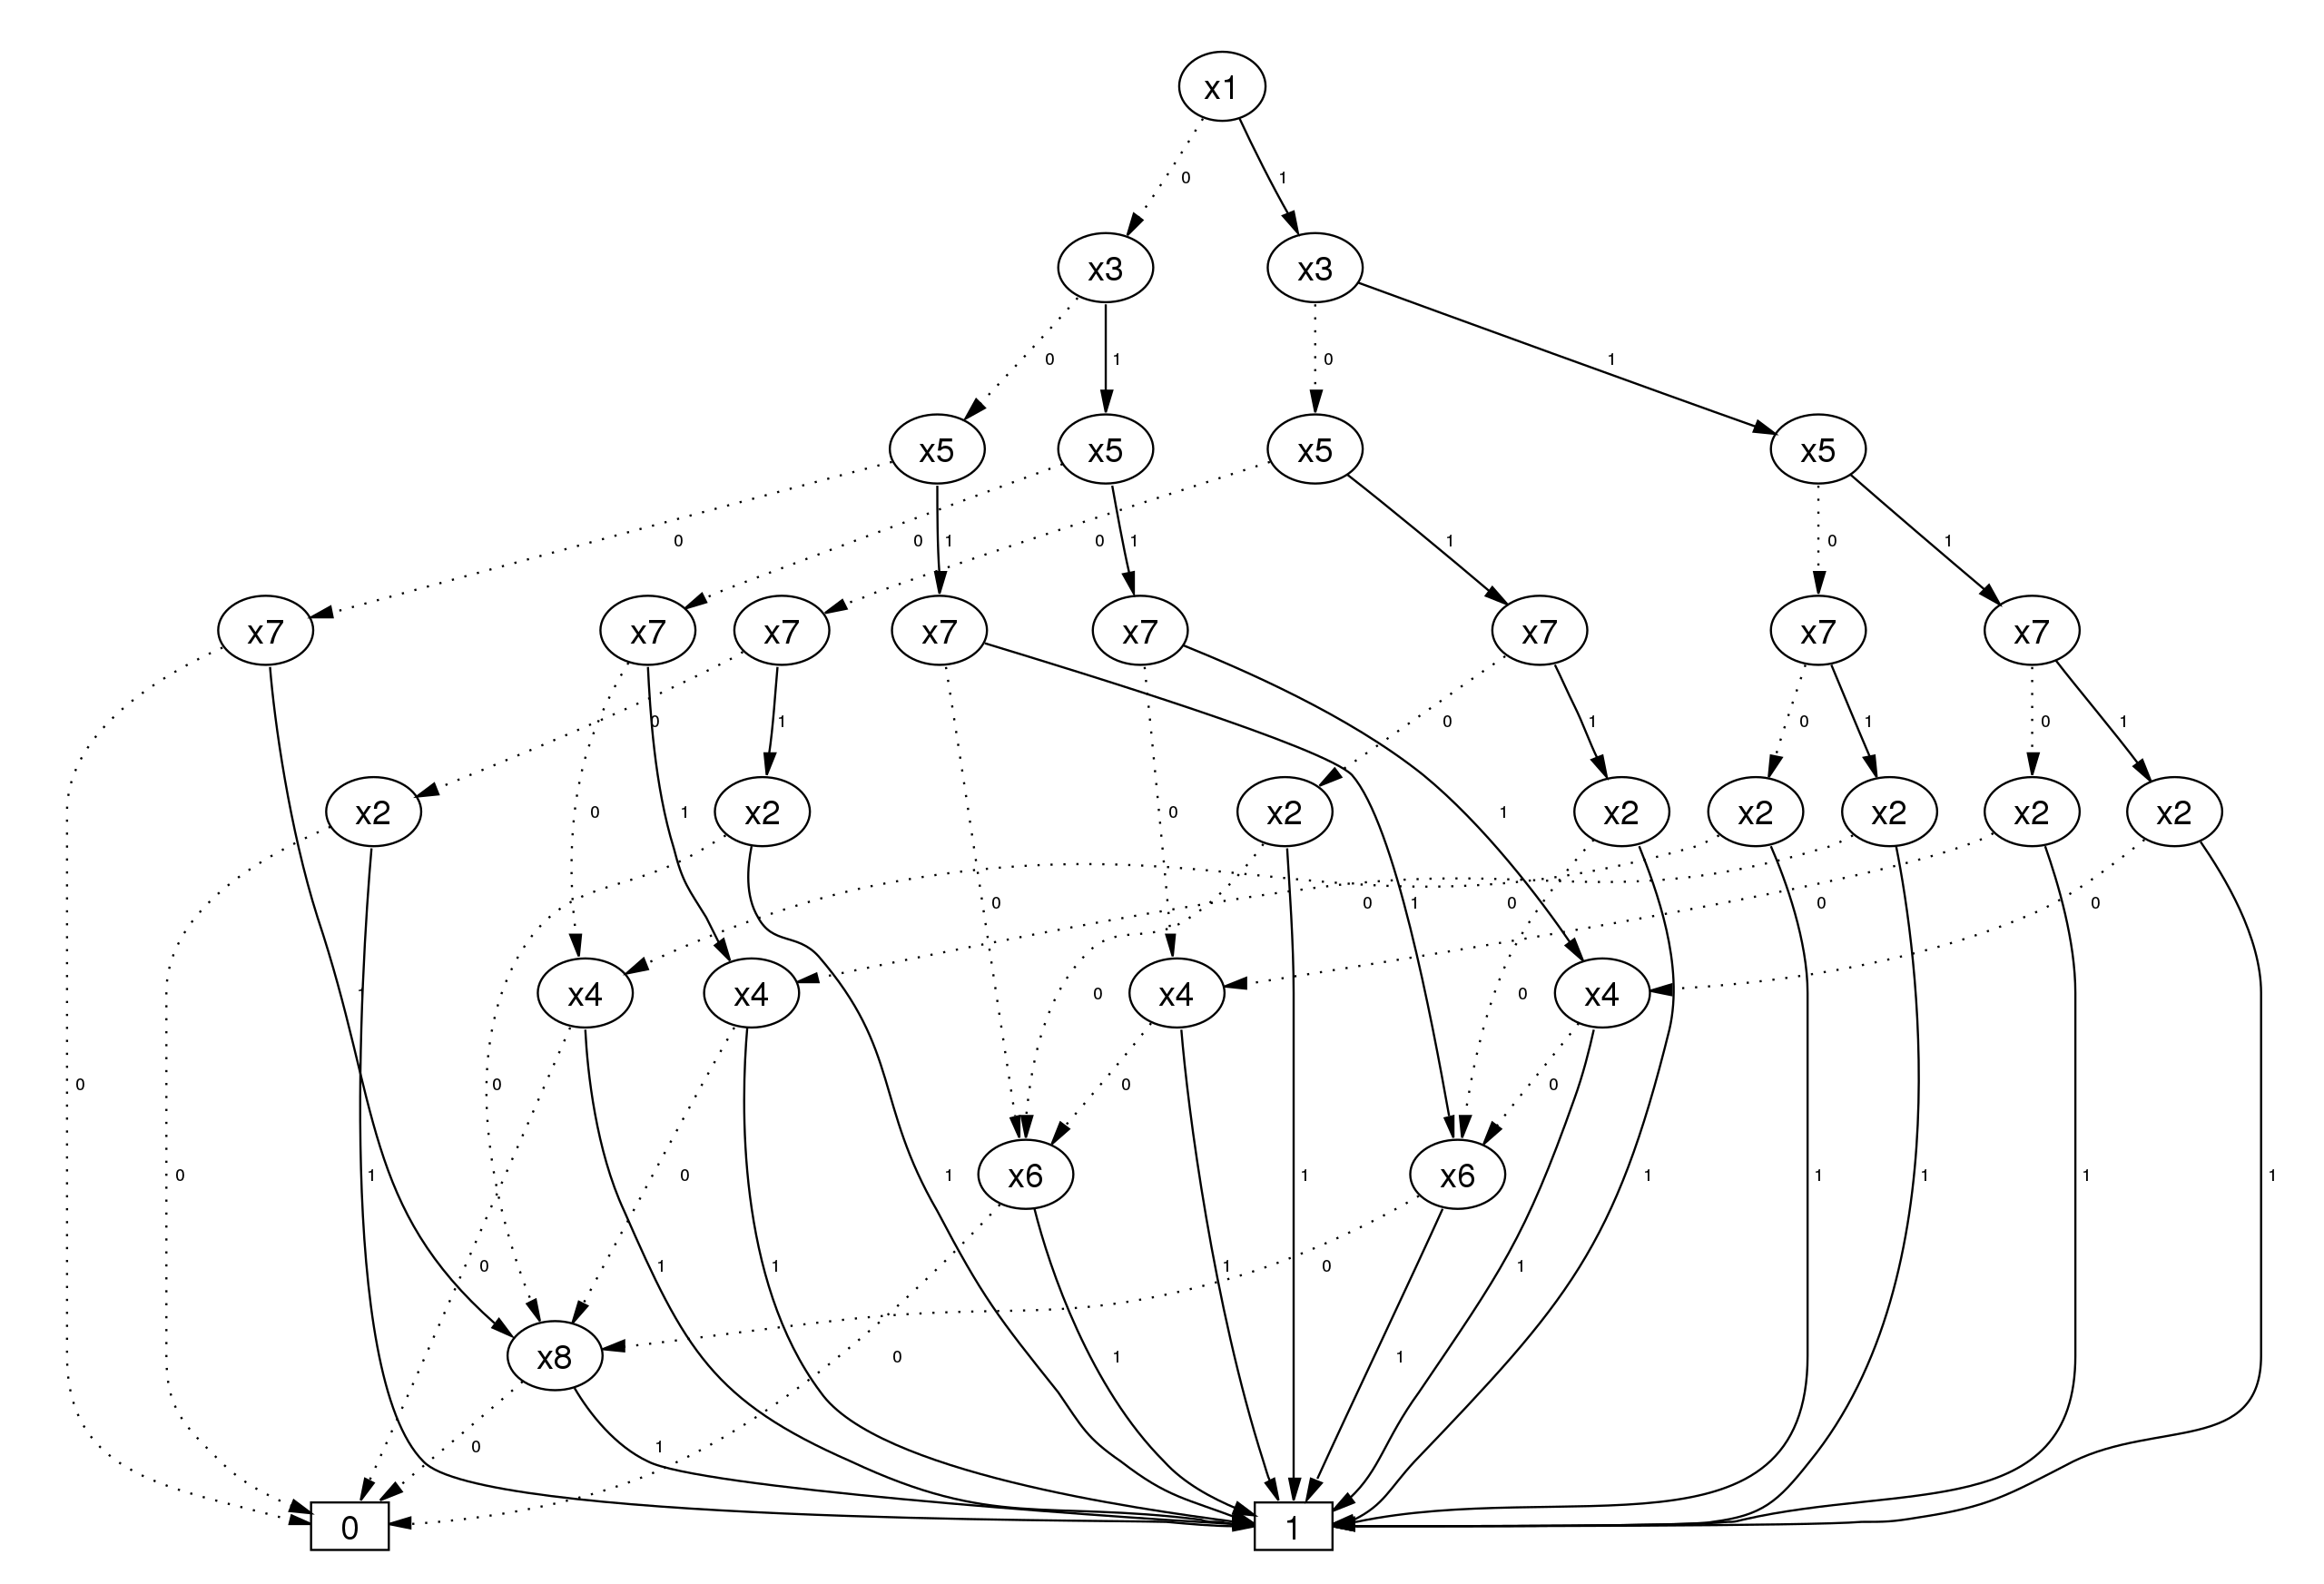
\includegraphics[height=6cm]{Img/BDD_Variable_Ordering_Bad.svg.pdf}
		\caption{索引顺序为\{x1,x3,x5,x7,x2,x4,x6,x8\}}
		\label{fig:bdd-bad}
	\end{subfigure}
    \qquad
	\begin{subfigure}[b]{.4\textwidth}
        \centering
        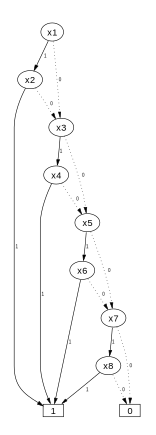
\includegraphics[height=6cm]{Img/BDD_Variable_Ordering_Good.svg.pdf}
		\caption{索引顺序为\{x1,x2,x3,x4,x5,x6,x7,x8\}}
		\label{fig:bdd-good}
	\end{subfigure}
	\caption{同一布尔函数在不同索引顺序下的结构图\citep{wiki:bdd}}
	\label{fig:bdd-compare}
\end{figure}


\item 由于量子状态都在同一希尔伯特空间中。因此作用某些算子后,不同的量子状态可能等价。
当存储算子的资源少于存储状态的资源时,就有可能存储算子表示不同的状态\citep{vinkhuijzen2023limdd}。图\ref{fig:qmdd-example}表示了一个QMDD的例子,应用等价性,可以化简为图\ref{fig:limdd-example}。
TDD也可以应用类似技术,进行进一步化简,从而降低资源要求。
\begin{figure}[!htbp]
    \centering
    \begin{subfigure}[b]{.4\textwidth}
        \centering
        \includegraphics[height=8cm]{Img/limdd.pdf}
        \caption{一个QMDD示例}
        \label{fig:qmdd-example}
    \end{subfigure}
    \begin{subfigure}[b]{.4\textwidth}
        \centering
        \includegraphics[height=8cm]{Img/limdd_reduce.pdf}
        \caption{应用等价性化简图\ref{fig:qmdd-example}}
        \label{fig:limdd-example}
    \end{subfigure}
\end{figure}
\end{myen}
\subsection{软件系统实现}
为了实现软件的高效运行,模块化设计至关重要。
每个模块在软件系统中扮演着关键角色,并且具有特定的功能和目的。以下是本次毕业设计中软件必须包含的模块及其重要性的说明:

\begin{itemize}
    \item \textbf{输入处理模块}:该模块的主要职责是处理输入数据,例如接收用OpenQASM格式编写的量子算法代码。其核心功能是将这些代码转换为TDD表示形式。鉴于当前存在多种量子编程语言,此模块的模块化处理能够显著提升系统的灵活性和兼容性。
    \item \textbf{内存管理模块}:本模块负责管理TDD节点的存储和维护。当创建新的TDD节点时,它会运用哈希算法与现有节点进行对比,以避免重复创建相同节点。这种方法不仅减少了内存占用,还提高了处理效率。
    \item \textbf{TDD基础模块}:该模块主要执行TDD节点的压缩操作,或者导出TDD的树状结构图。节点收缩是TDD核心的运算过程,而树状结构图的导出功能则有助于用户更好地理解和分析TDD的结构。
    \item \textbf{TDD算法模块}:此模块为TDD提供更复杂的算法支持。例如,它能够调整节点收缩的顺序,以优化系统运行效率。此外,它还能执行其他高级功能,如检验TDD是否存在于特定子空间中。
\end{itemize}